\documentclass[a4paper,10pt]{article}
\usepackage[utf8]{inputenc}
\usepackage[margin=1in]{geometry}
\usepackage{graphicx}

%opening


\begin{document}


\begin{figure}[h!]
 \centering
 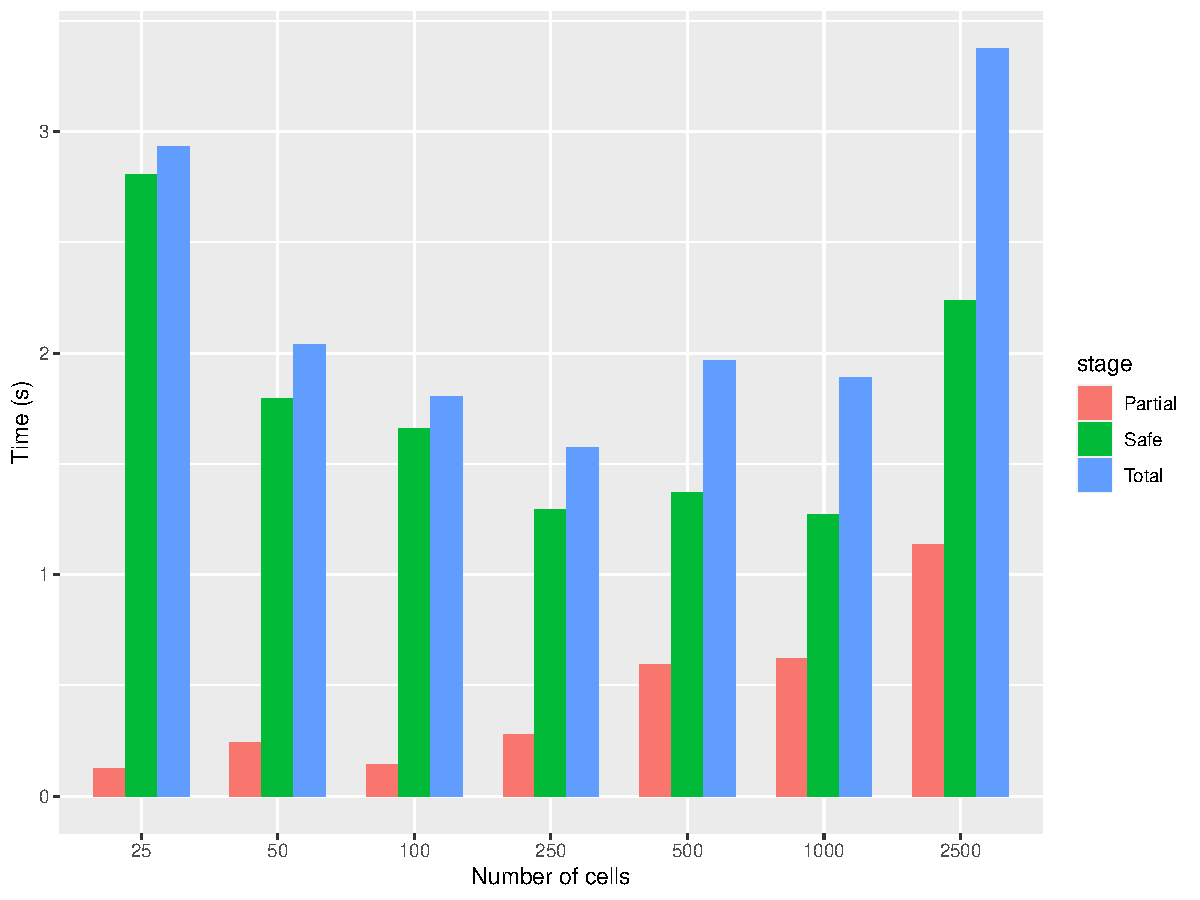
\includegraphics[width=0.9\textwidth]{berlinE30_partitions.pdf}
 \caption{Berlin $\varepsilon$ = 30m}
 \label{fig:berlin30}
\end{figure}

\begin{figure}[h!]
 \centering
 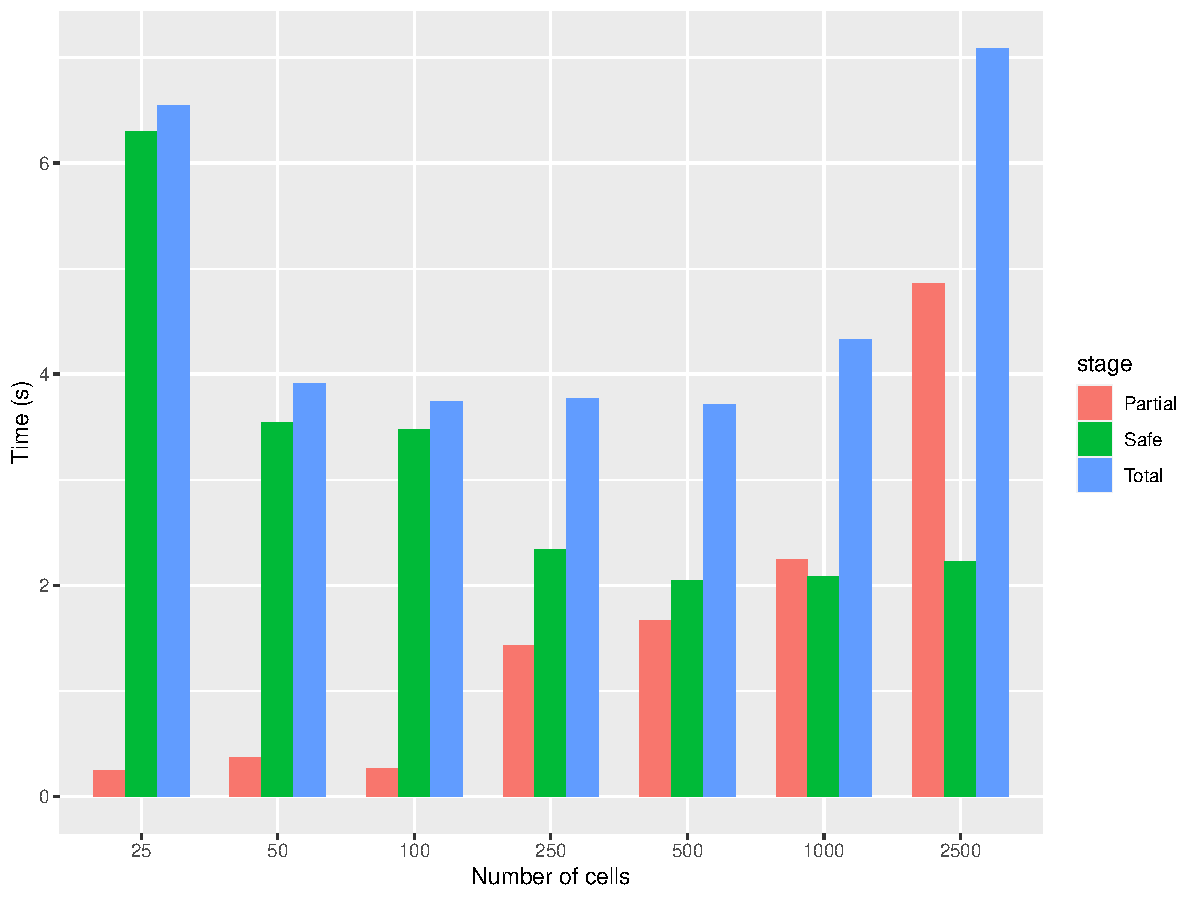
\includegraphics[width=0.9\textwidth]{berlinE40_partitions.pdf}
 \caption{Berlin $\varepsilon$ = 40m}
 \label{fig:berlin40}
\end{figure}

\begin{figure}[h!]
 \centering
 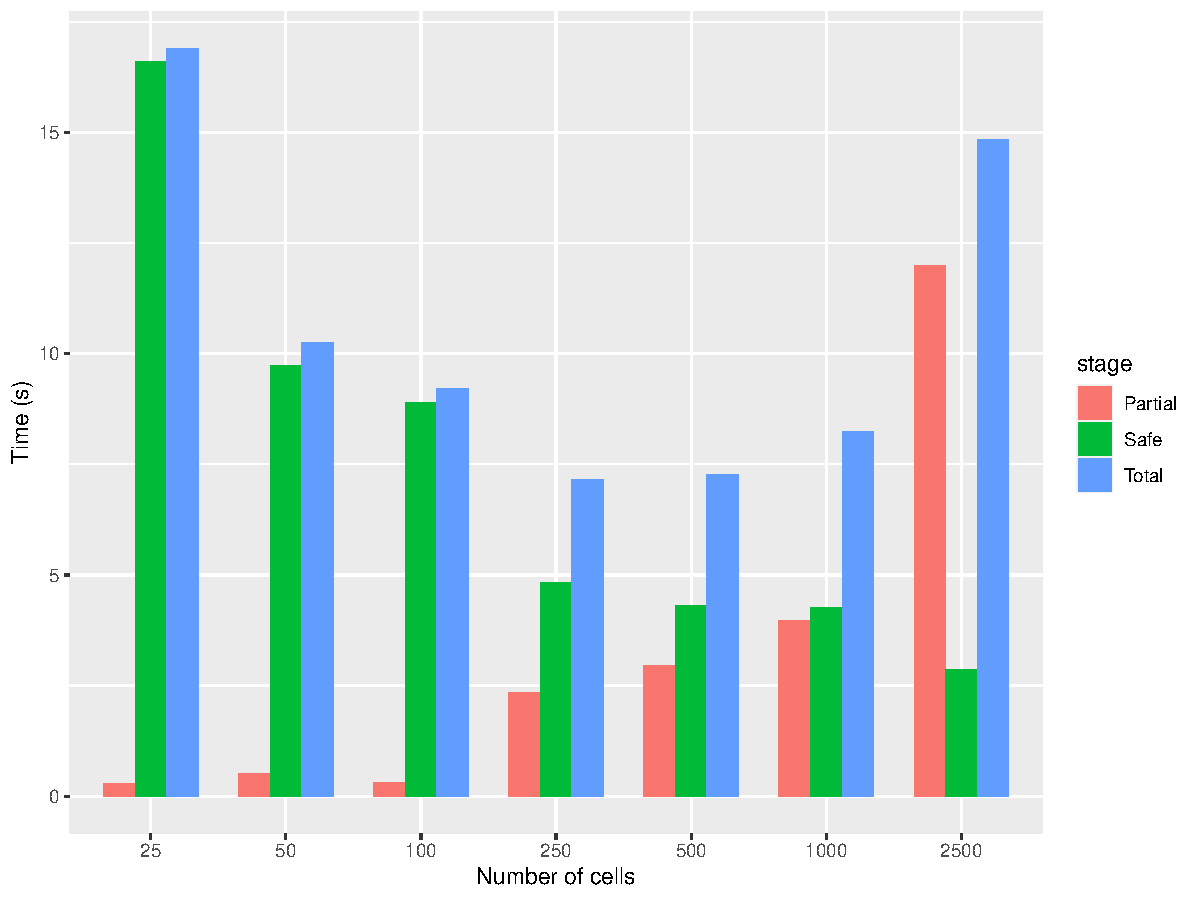
\includegraphics[width=0.9\textwidth]{berlinE50_partitions.pdf}
 \caption{Berlin $\varepsilon$ = 50m}
 \label{fig:berlin50}
\end{figure}

\begin{figure}[h!]
 \centering
 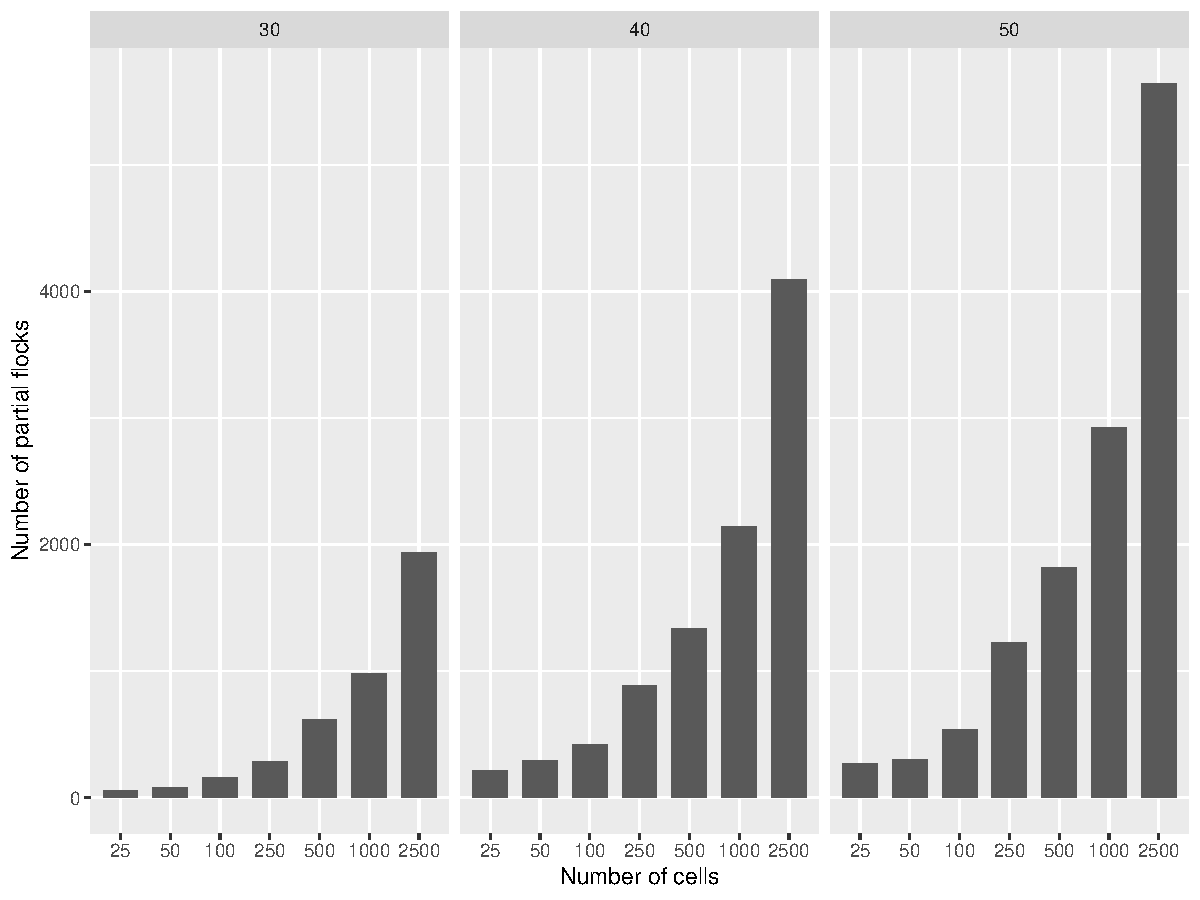
\includegraphics[width=0.9\textwidth]{berlin_npartials.pdf}
 \caption{Berlin - Number of partial flocks in crest}
 \label{fig:berlin_npartials}
\end{figure}



\begin{figure}[h!]
 \centering
 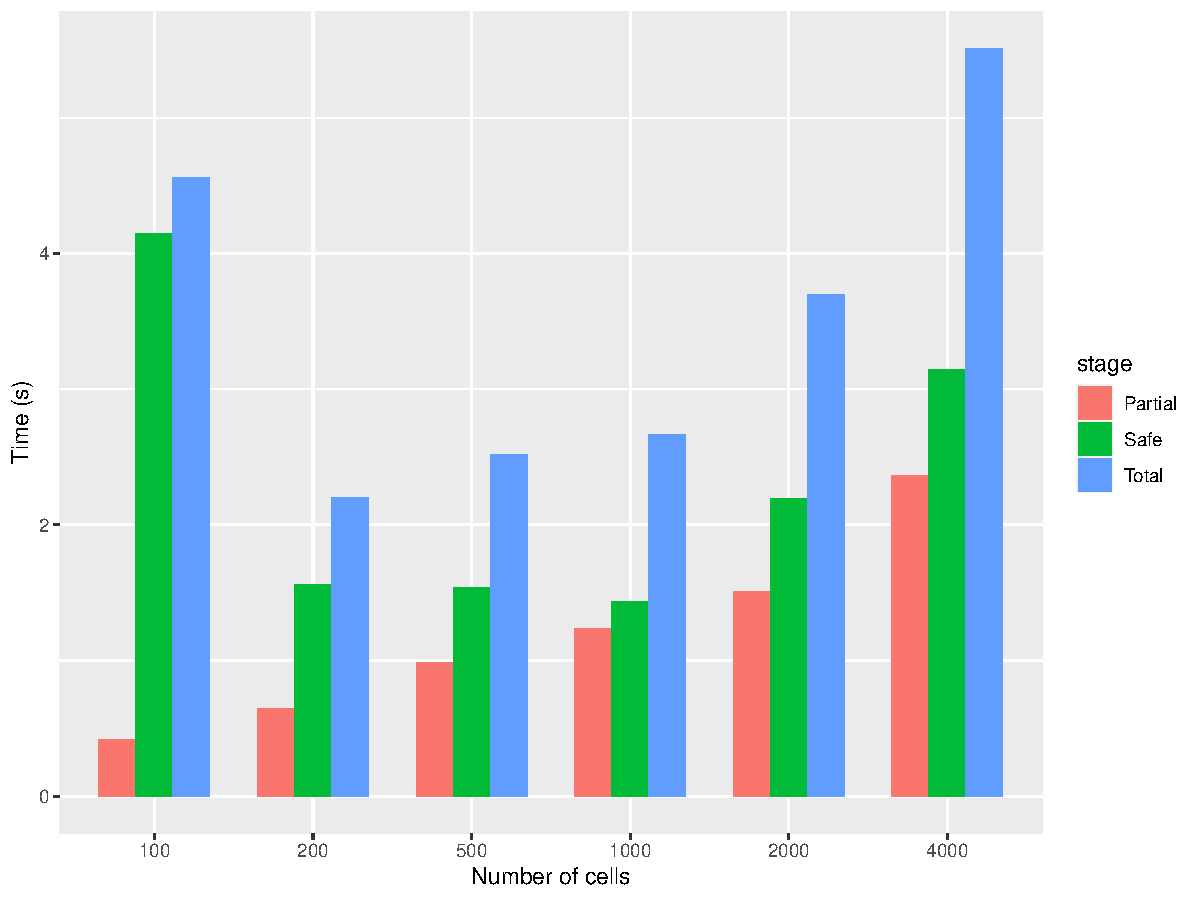
\includegraphics[width=0.9\textwidth]{la25kE10_partitions.pdf}
 \caption{LA25K $\varepsilon$ = 10m}
 \label{fig:la25k10}
\end{figure}

\begin{figure}[h!]
 \centering
 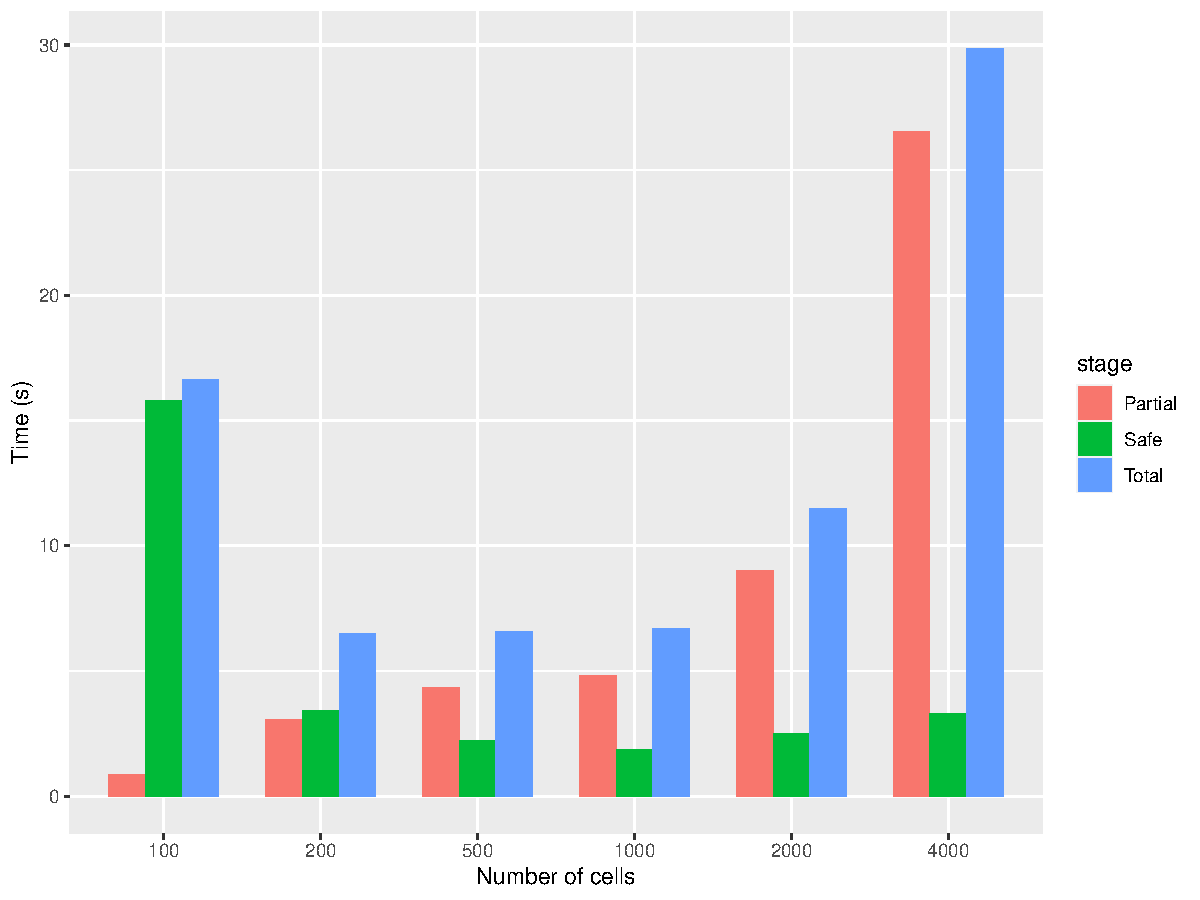
\includegraphics[width=0.9\textwidth]{la25kE15_partitions.pdf}
 \caption{LA25K $\varepsilon$ = 15m}
 \label{fig:la25k15}
\end{figure}

\begin{figure}[h!]
 \centering
 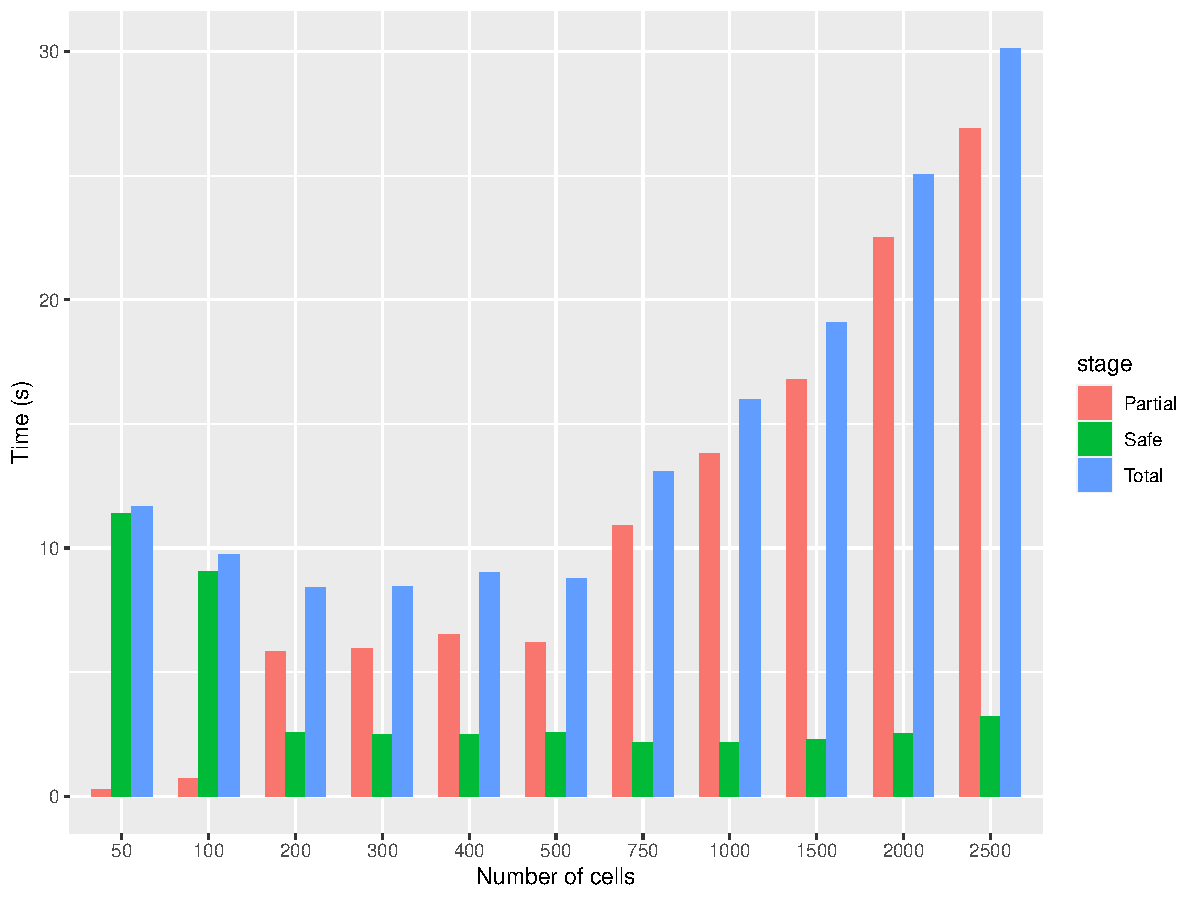
\includegraphics[width=0.9\textwidth]{la25kE20_partitions.pdf}
 \caption{LA25K $\varepsilon$ = 20m}
 \label{fig:la25k20}
\end{figure}

\begin{figure}[h!]
 \centering
 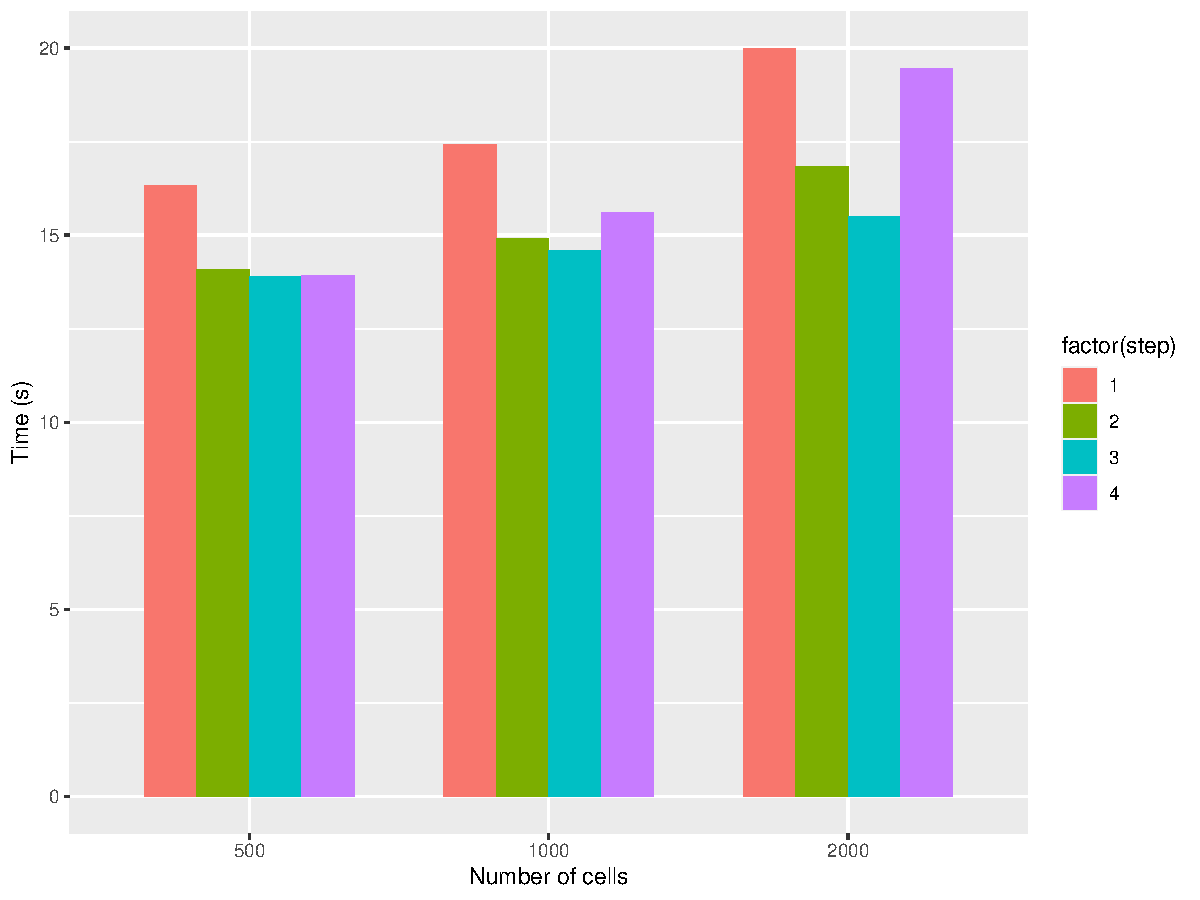
\includegraphics[width=0.9\textwidth]{la25k_steps.pdf}
 \caption{LA25K - Incremental partial flock processsing}
 \label{fig:la25k_steps}
\end{figure}

\end{document}
